\subsection{Overview}
The following diagram represents the high level architecture of the system, including the external entities that will interact with it.
\\
\begin{figure}[H]
    \centering
    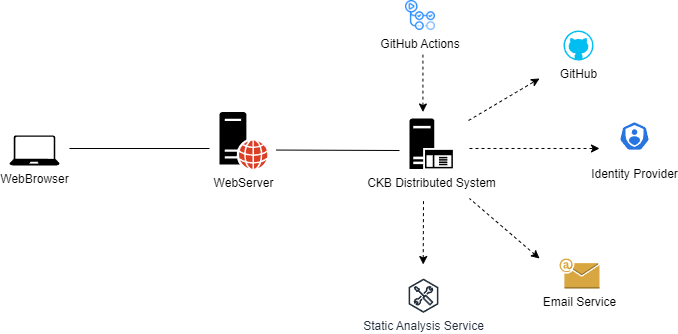
\includegraphics[width=1\textwidth]{Diagrams/overview.png}
    \caption{CKB system diagram}
    \label{overview_diagram}
\end{figure}
The main elements contained in Figure \ref{overview_diagram} are:
\begin{itemize}
    \item \textbf{WebBrowser} used by students and educators to access the system functionalities through the web application.
    \item \textbf{WebServer} whose functions are:
    \begin{itemize}
        \item Serving static assets (HTML, CSS, JavaScript) to the client, necessary for handling the initial rendering of the UI.
        \item Managing the client-side application and routing.
        \item Generating requests directed to the backend system.
    \end{itemize}
    \item \textbf{CKB Distributed System} which is the distributed system composed of multiple microservices that implement the core functionalities of the system. Its in charge of the data management, application and integration logic of the whole CKB platform.
    \item \textbf{External Entities} the CKB Distributed System must be able to integrate with to accomplish its functionalities. The arrow in the diagram highlights the direction of the interaction between the system and the external entities.
\end{itemize}

\subsection{Component view}
The following component diagram highlights the main components of the system and their interaction with external entities and services. In the diagram, the components have been organized to highlight the logical grouping of the system elements.

The WebApplication component represents the presentation layer of the system, being the only entry point for the users. The application and integration logics are represented together due to their tight interaction, while the data layer contains the databases accessed by the respective microservices.

Different colors are used to highlight components that share similar roles in the system.
\begin{itemize}
    \item \textcolor{orange}{Orange} components represent the system's microservices. Complex microservices have been further decomposed into subcomponents, for a more fine grained representation. Some microservices have an important role in the integration and communication with external entities as well, but have been depicted with their orange color used for microservices. This aspect will be clarified in the detailed description of the components that follows the diagram.
    \item \textcolor{myyellow}{Yellow} components represent the model of the database accessed by its microservice. The model offers to the microservice an abstraction of the database, allowing it to access the data without knowing the underlying database implementation technology.
    \item \textcolor{violet}{Violet} has been used to highlight components or services that cover an important role for the communication between microservices. It has been used for the queues subcomponents, which are used to implement the asynchronous and concurrent communication between specific microservices. Also the ServiceRegistry has been represented with the this color, since it enables the communication in the system. It's important to notice that for the sake of simplicity and readability, the interface offered by the ServiceRegistry has been depicted with some dotted arrows that connect all the microservices to it.
    \item \textcolor{red}{Red} components represent the external services that interact with the system.
    \item Finally, the \textcolor{mygreen}{green} color has been used to highlight the databases components that are used to store the data of the system.
\end{itemize}

\newpage
\thispagestyle{noheader}
\begin{figure}[H]
    \centering
    \vspace{-3.5cm}
    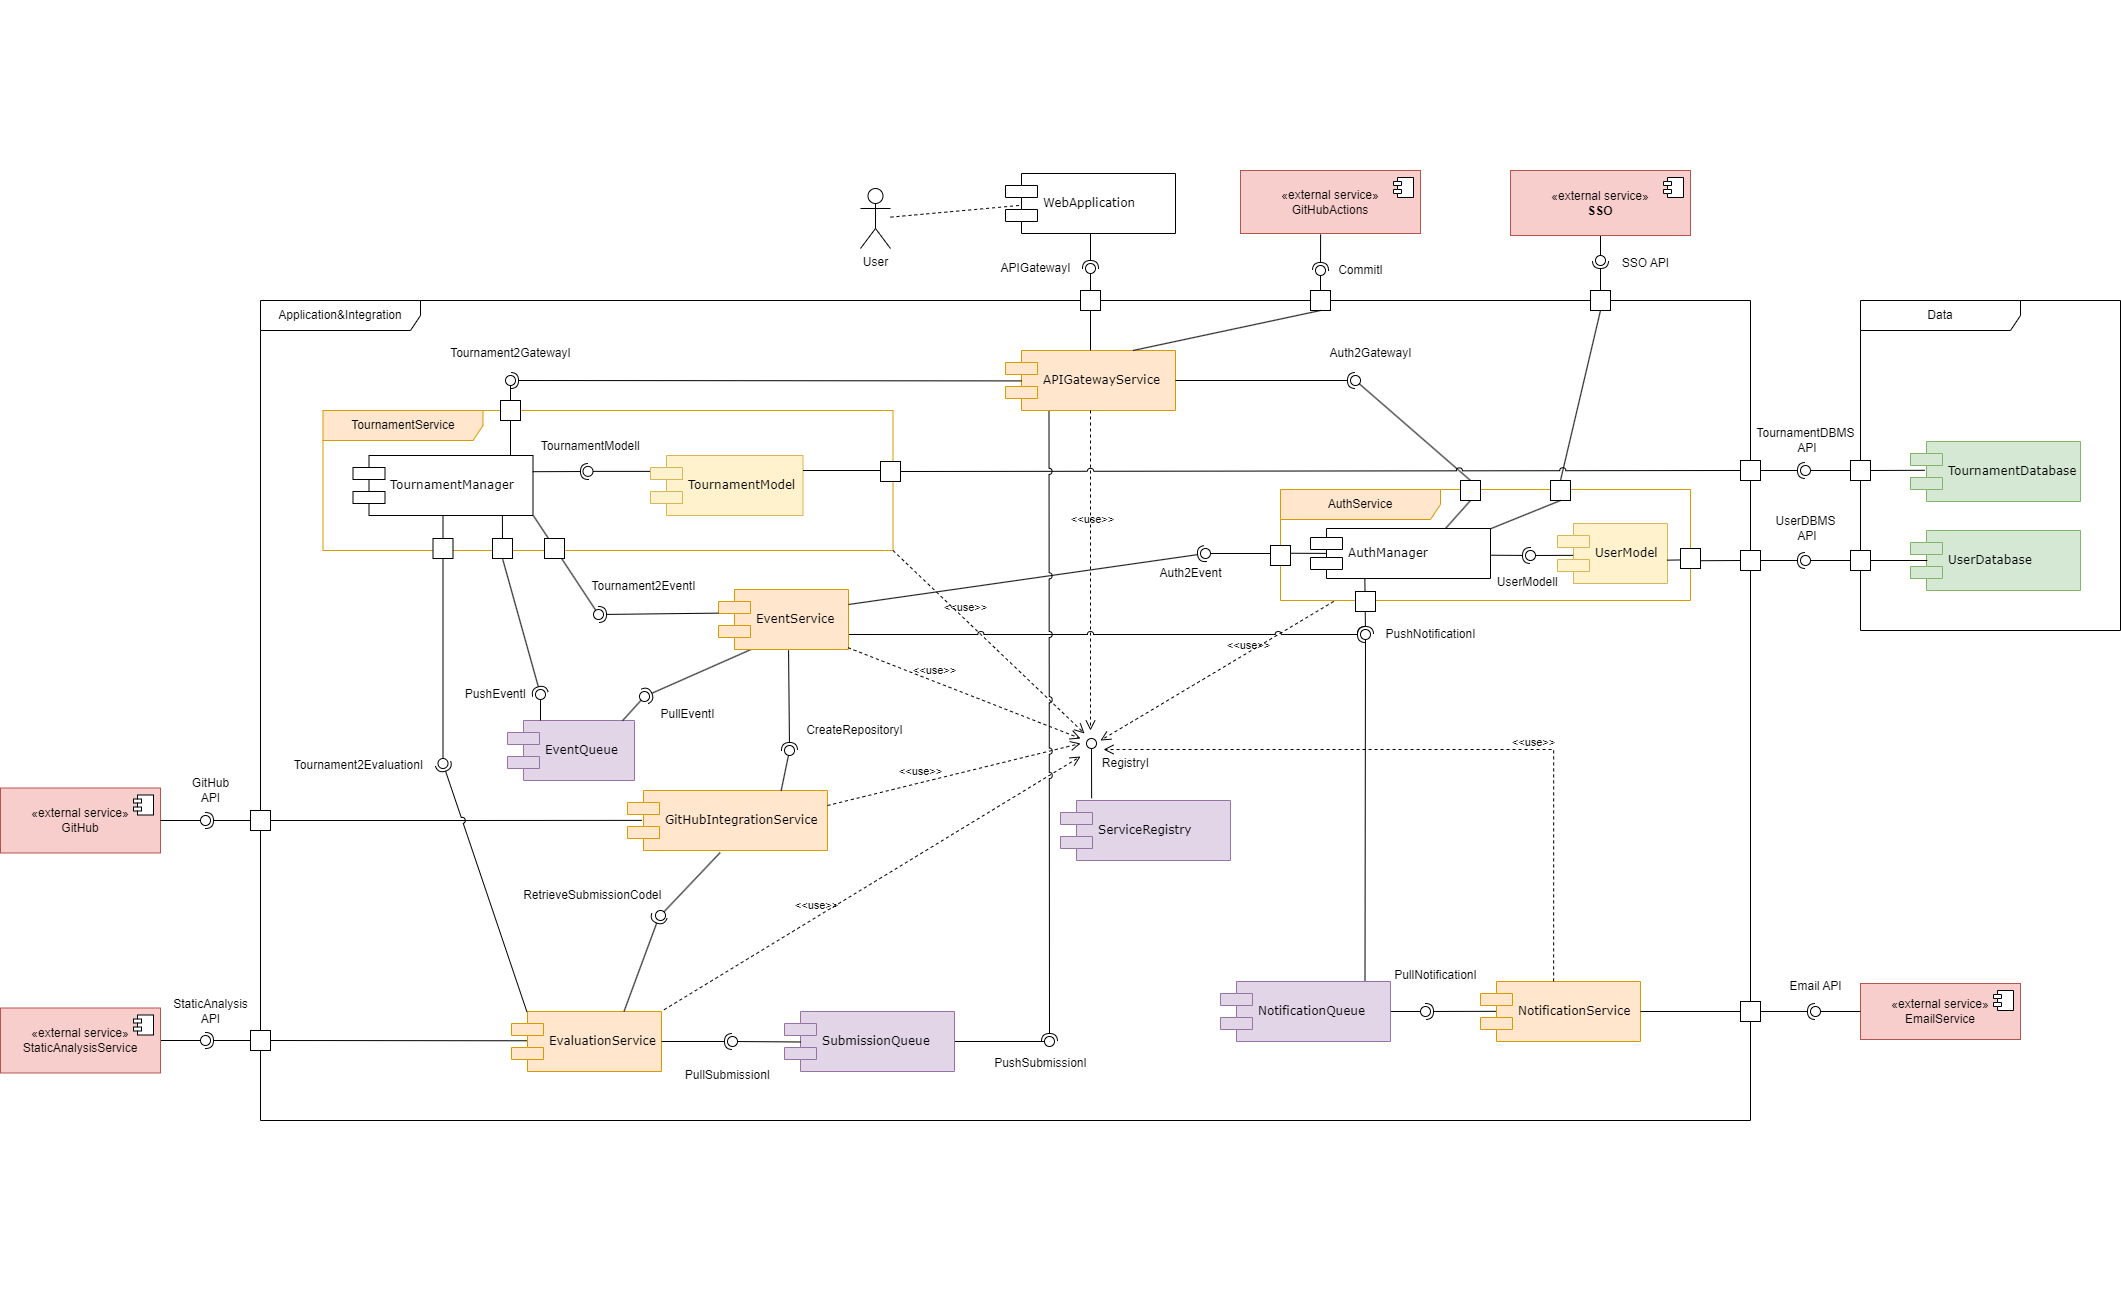
\includegraphics[width=1.6\textwidth,angle=90,origin=c]{Diagrams/component_diagram.png}
    \caption{Component diagram}
    \label{component_diagram}
\end{figure}

The components in Figure \ref{component_diagram} are :
\begin{itemize}
    \item \textbf{WebApplication}: the web app to which users of the CKB platform (students and educators) connect through a modern web browser. It is the front end of the system, and thanks to the interface offered by the \textbf{APIGatewayService}, allows users to manage and access the most important aspects of tournaments and battles.
    \item \textbf{APIGatewayService}: this component is the microservice that exposes the REST API used by the WebApplication. Indeed, it allows the implementation of the main functionalities needed by the users of the web application by orchestrating the microservices. It also offers a REST API, used by the GitHub Actions Service, to notify a submission of a student on the Github repository.
    It's also responsible for the following functionalities:
    \begin{itemize}
        \item Acts as a single entry point for client requests.
        \item Handles authentication, authorization through the interaction with the AuthService.
        \item Routes requests to the appropriate microservices that provide the required business functionality.
        \item Aggregates responses from multiple microservices if needed.
        \item Load balancing and API rate limiting.
    \end{itemize}
    \item \textbf{AuthService}: this component is the microservice that handles the authentication of the users of the system. To accomplish this task, it may be required to interact with external identity providers, depending on the user preferences. 
    It is responsible also for all the data related to the users of the system, such as their personal information and their roles. It includes the following subcomponents:
    \begin{itemize}
        \item \textbf{AuthManager}: implements the main logical functionalities of the AuthService, exposing APIs used by other microservices to authenticate and to retrieve user information.
        \item \textbf{UserModel}: represents the model of the database used by the AuthService to store the data related to the users of the system.
    \end{itemize}
    \item \textbf{TournamentService}: this component is the microservice that implements most of the functionalities needed by the users. It handles:
    \begin{itemize}
        \item Management of tournaments and battles: it allows the creation of battle and tournaments, enrollment of students to tournaments and battles.
        \item Management of events regarding tournaments and battles.
        \item Management of the ranking of the students.
        \item Management of data related to tournaments, battles and submissions
        \item Manual evaluation of the submissions of the students.
    \end{itemize}
    It is composed of the following subcomponents:
    \begin{itemize}
        \item \textbf{TournamentManager}: implements the main logical functionalities of the TournamentService, exposing APIs used by other microservices to manage tournaments and battles and their data.
        \item \textbf{TournamentModel}: represents the model of the database used by the TournamentService to store the data related to tournaments and battles.
        \item \textbf{EventManager}: periodically checks the EventQueue for events and processes them once the deadlines are reached.
    \end{itemize}
    \item \textbf{GitHubIntegrationService}: this component is the microservice that handles the integration with GitHub. It is responsible for the following functionalities:
    \begin{itemize}
        \item Creation of the GitHub repository of the battle.
        \item Retrieval of the code of the submission from the GitHub repository.
    \end{itemize}
    \item \textbf{EvaluationService}: this component is the microservice that handles the evaluation of the submissions of the students. It periodically checks the SubmissionQueue for submissions to evaluate and processing them. The submission notification contains only the token associated to the team, so the service retrieves the code from the GitHub repository, interacting with the GitHubIntegrationService.
     This service is responsible for the following functionalities:
    \begin{itemize}
        \item Evaluation of the submissions, in terms of timeliness and functional analysis 
        \item Integration with external static code analysis tools to evaluate the quality of the code of the submissions.
    \end{itemize}
    \item \textbf{NotificationService}: this component is the microservice that handles the notifications of the users of the system. It periodically checks the NotificationQueue for new notifications to send and processing them. To perform this task, the NotificationService interacts with the external email service provider to send notifications to the users.
     It is responsible for the following functionalities:
    \begin{itemize}
        \item Dispatch of confirmation email to new registered users.
        \item Dispatch of email notifications to users in case of events related to tournaments and battles.
    \end{itemize}
    In the diagram, this component has not been connected to the ServiceRegistry, since it is a standlone service that does not need to synchronously communicate with the other microservices (communication with others microservices is asynchronous and relies only on the NotificationQueue).
    \item \textbf{ServiceRegistry}: this component handles the registration of the microservices to the system. It offers to all the microservices the following:
    \begin{itemize}
        \item Registration of the microservices istances to the system.
        \item Discovery of the microservices istances by the other microservices.
        \item Availability check of the microservices istances, by receiving periodic heartbeats from them.
    \end{itemize}
    \item \textbf{TournamentDatabase}: this component is the database used by the system to store the data related to tournaments and battles, including also scores and ranks.
    \item \textbf{UserDatabase}: this component is the database used by the system to store the data related to the users of the system, such as kind of user, email and usernames.
    \item \textbf{NotificationQueue}: queue that stores new notifications to be dispatched.
    \item \textbf{SubmissionQueue}: queue that stores notifications about new pending submissions, appended by the GitHubActions through the REST API exposed by the APIGatewayService, yet to be evaluated.
    \item \textbf{EventQueue}: the queue used by the TournamentService to manage the events related to tournaments and battles. It is implemented as a priority queue, so that events are ordered by their deadlines.
\end{itemize}
The Figure \ref{component_diagram} contains also some external entities the system interacts with:
\begin{itemize}
    \item \textbf{GitHub}: used by the system to retrieve the code of GitHub repositories and to create new repositories.
    \item \textbf{GitHubActions}: configured by the students on their GitHub repository to automatically notify the system when a new submission is pushed to the repository.
    \item \textbf{StaticAnalysisService}: used by the system to evaluate the quality of the code of the submissions.
    \item \textbf{EmailService}: used by the system to send emails to the users of the system.
    \item \textbf{SSO}: used by the system to offer the users the possibility to signup and login with their preferred identity provider.
\end{itemize}

\newpage
\subsection{Deployment view}
The following diagram represents the deployment architecture of the system, highlighting the physical nodes on which the system will be deployed and the communication channels between them.

In Figure \ref{deployment_diagram} the nodes have been colored according to the color scheme defined in the component view exception, with the only difference that the \textcolor{red}{red} color has been used to identify the user's web browser and the \textcolor{myyellow}{yellow} one to represent the system's web server.

The most important aspects that are worth noticing are:
\begin{itemize}
    \item Queues are deployed on a single phisical node. As we can see from the artifacts, all queues are built over the same code but replicated in a way that each type of microservice uses its own: this should increase modularity and maintainability of the system. Moreover these queues are logged (i.e. also persisted in secondary memory) so that, in case of failure, a new service can be deployed and the previous state of the queue can be restored: this allows the system to be fault tolerant by ensuring that no communication data is lost.
    \item Most of the microservices are deployed in a containerized environment, using Docker containers. This allows them to be easily deployed on necessity, allowing the system to scale out according to the current load. The Service Registry instead is deployed in a non-containerized environment, since it is a critical component of the system and it is important to ensure its availability. In particular, in order to achieve this, a master-slave approach has been chosen. The master instance is deployed on a physical node, while slave instances are deployed on different nodes: the latter ones have the task of monitoring the master instance and to copy its logs. In this way, if the master instance fails, one of the slave instances (e.g. chosen through a consensus algorithm) can be promoted to master so the system can continue to work from the point the master left without any interruption.
\end{itemize}
\begin{figure}[H]
    \centering
    \vspace{-4cm}
    \hspace{1cm}
    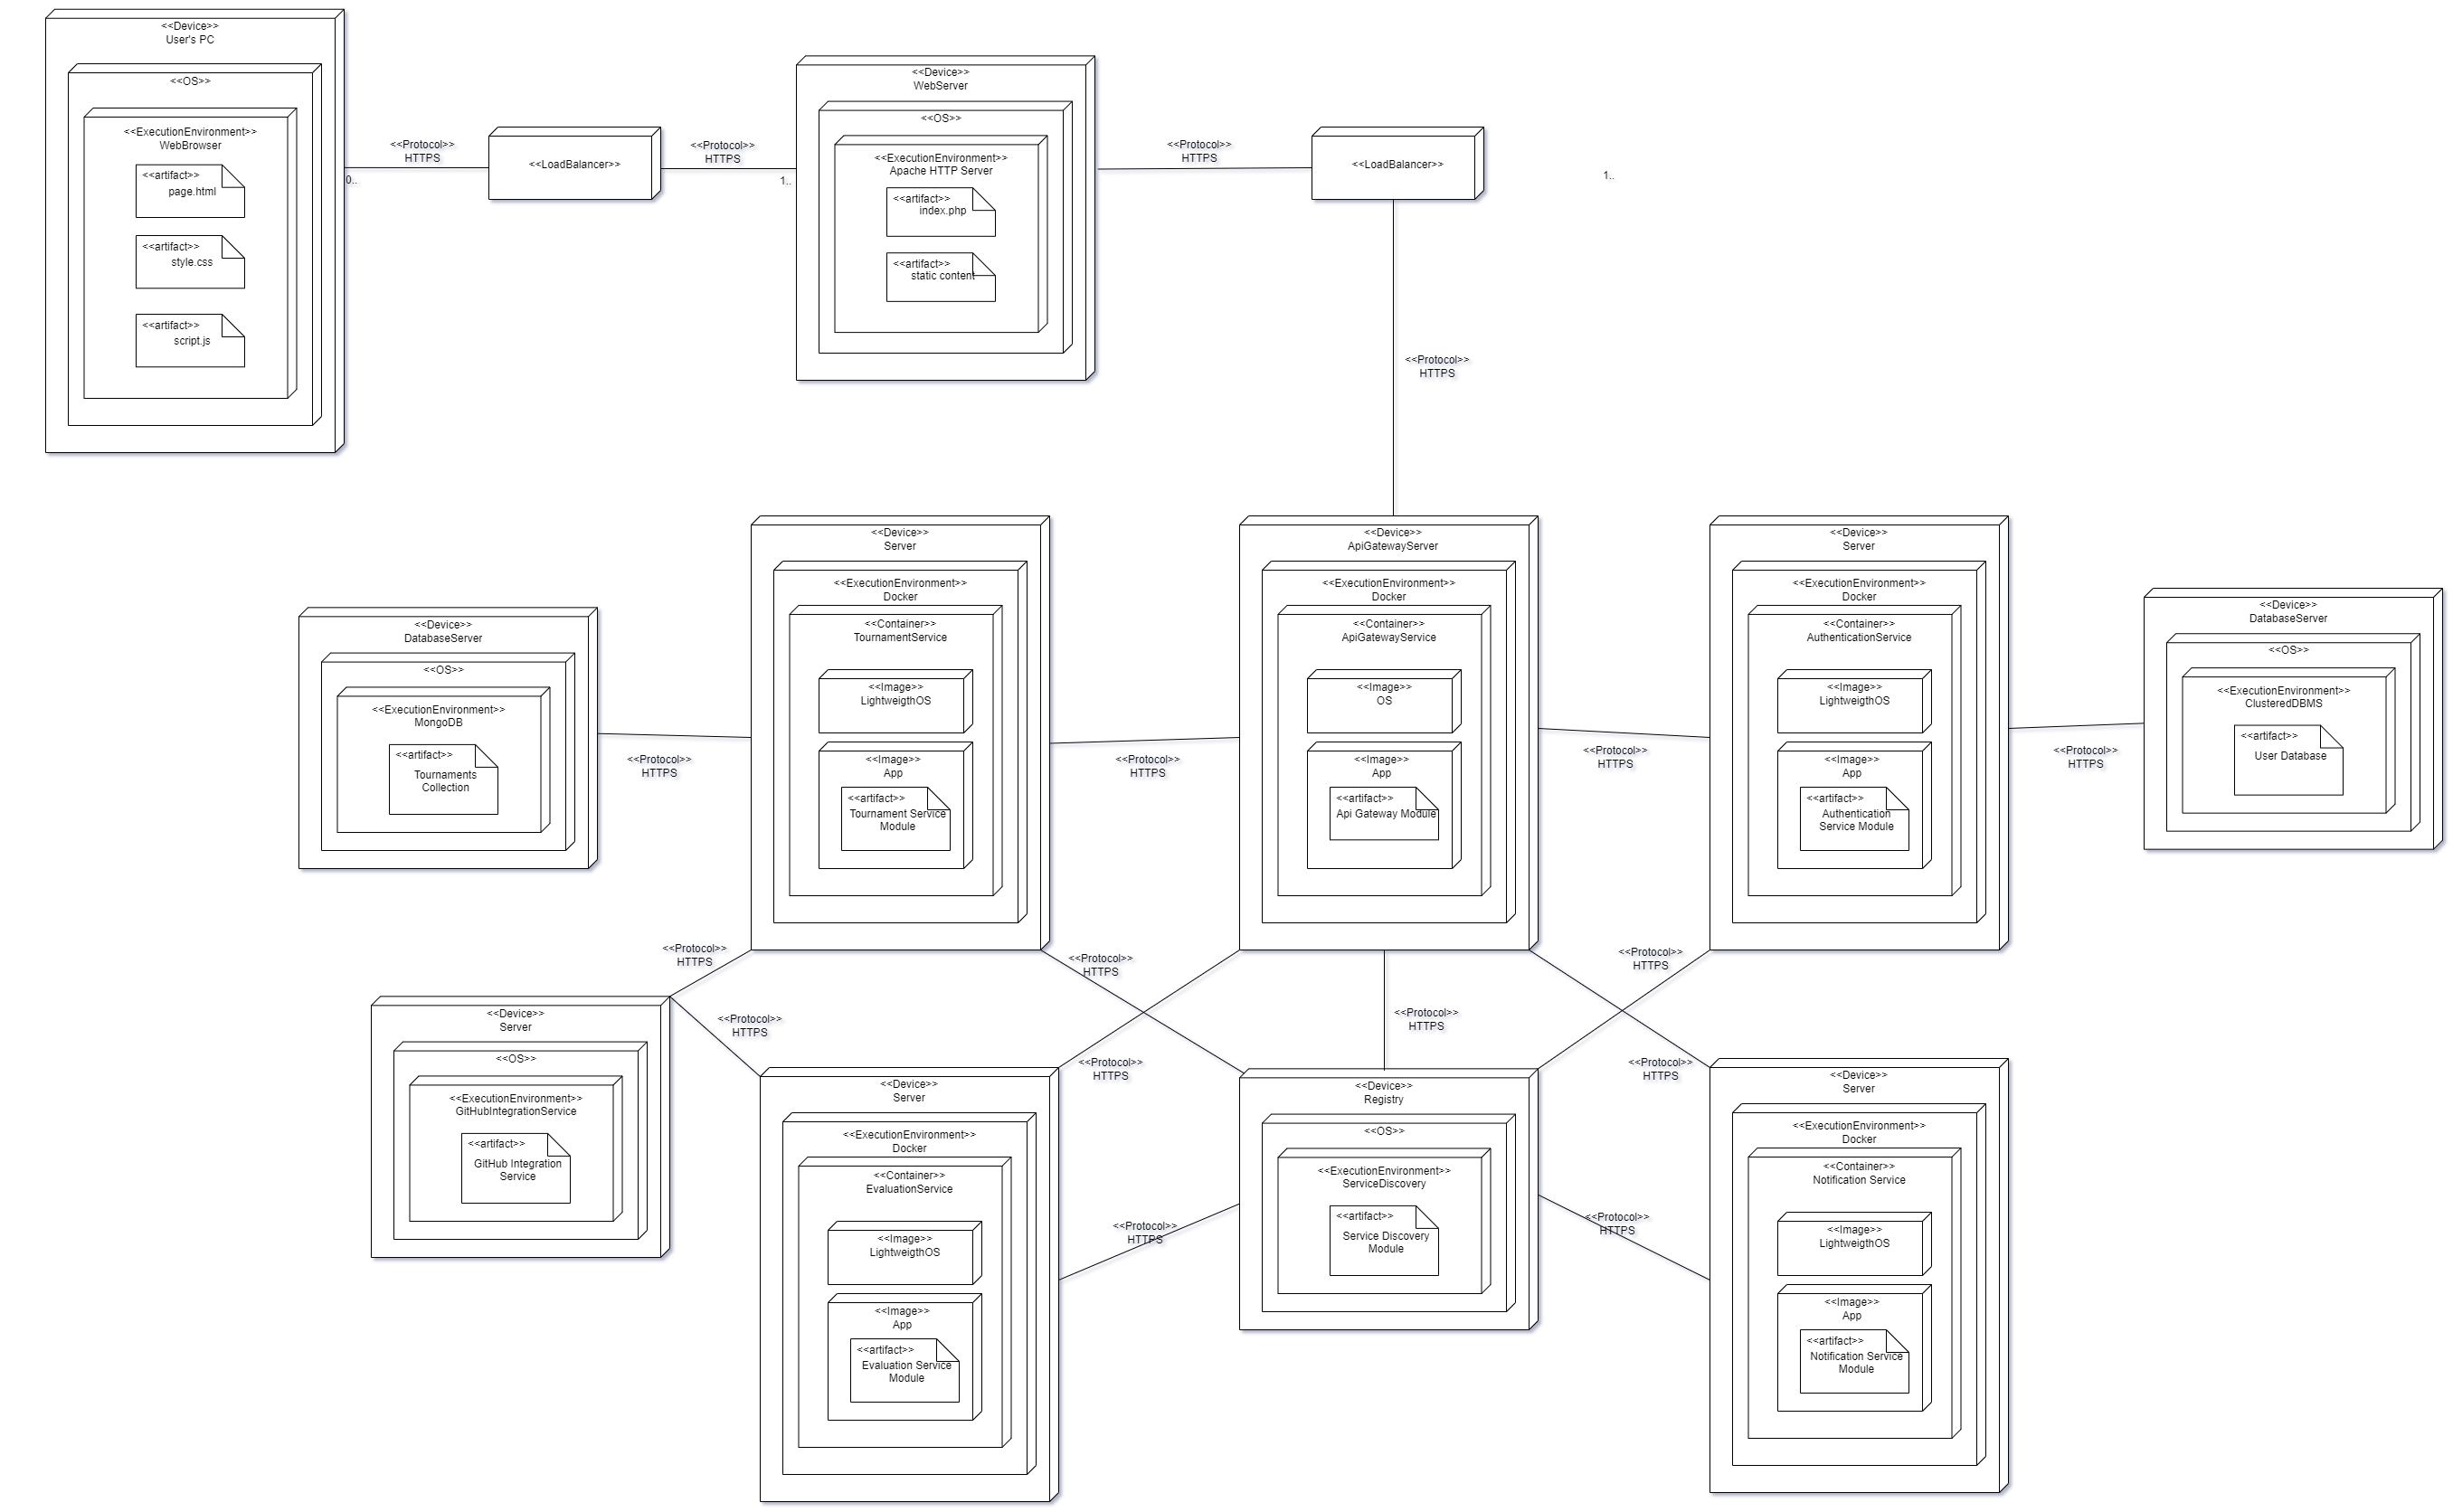
\includegraphics[width=1.1\textwidth]{Diagrams/deployment_diagram.png}
    \caption{Deployment diagram}
    \label{deployment_diagram}
\end{figure}

\subsection{Component interfaces}
In this section the interfaces of the components of the system are described. The interfaces are described in terms of the operations they offer and the parameters they require and return.\\

\begin{itemize}
    \item \textbf{APIGatewayI}
    \begin{itemize}
        \item login(credentials): bool
        \item signup(credentials): bool
        \item initializeLoginSSO(identityProvider): none
        \item completeLoginSSO(identityProvider,ssoToken): bool
        \item initializeSignupSSO(identityProvider): none
        \item completeSignupSSO(identityProvider,ssoToken): bool
    \end{itemize}
    \item \textbf{Auth2GatewayI}
    \begin{itemize}
        \item authenticateUser(credentials): userId
        \item createUser(credentials): userId
        \item completeLoginSSO(identityProvider,ssoToken): userId
        \item completeSignupSSO(identityProvider,ssoToken): userId
    \end{itemize}
    \item \textbf{UserModelI}
    \begin{itemize}
        \item getUserId(credentials): userId
        \item createUser(credentials): userId
        \item createUserSSO(userData): userId
        \item getUserData(userId): userData
    \end{itemize}
    \item \textbf{Auth2TournamentI}
    \begin{itemize}
        \item 
    \end{itemize}
    \item \textbf{CommitI}
    \begin{itemize}
        \item 
    \end{itemize}
    \item \textbf{Auth2GatewayI}
    \begin{itemize}
        \item 
    \end{itemize}
    \item \textbf{Tournament2GatewayI}
    \begin{itemize}
        \item 
    \end{itemize}
    \item \textbf{Tournament2EventI}
    \begin{itemize}
        \item 
    \end{itemize}
    \item \textbf{Tournament2EvaluationI}
    \begin{itemize}
        \item 
    \end{itemize}
    \item \textbf{TournamentModelI}
    \begin{itemize}
        \item 
    \end{itemize}
    \item \textbf{PushEventI}
    \begin{itemize}
        \item 
    \end{itemize}
    \item \textbf{PullEventI}
    \begin{itemize}
        \item 
    \end{itemize}
    \item \textbf{CreateRepositoryI}
    \begin{itemize}
        \item 
    \end{itemize}
    \item \textbf{RetrieveSubmissionCodeI}
    \begin{itemize}
        \item 
    \end{itemize}
    \item \textbf{PullSubmissionI}
    \begin{itemize}
        \item 
    \end{itemize}
    \item \textbf{PushSubmissionI}
    \begin{itemize}
        \item 
    \end{itemize}
    \item \textbf{PushNotificationI}
    \begin{itemize}
        \item 
    \end{itemize}
    \item \textbf{PullNotificationI}
    \begin{itemize}
        \item 
    \end{itemize}
    \item \textbf{RegistryI}
    \begin{itemize}
        \item 
    \end{itemize}
\end{itemize}

The system's components will exploit the following APIs, provided by already existing services or components:
\begin{itemize}
    \item \textbf{TournamentDBMS API}: 
    \item \textbf{UserDBMS API}: 
    \item \textbf{GitHub API}: 
    \item \textbf{StaticAnalysis API}: 
    \item \textbf{Email API}:
    \item \textbf{SSO API}:
        \begin{itemize}
            \item retrieveUserInformation(ssoToken): userData
        \end{itemize}
\end{itemize}












\subsection{Runtime view}
\subsection{Selected architectural styles and patterns}
\subsection{Other design decisions}